% Compile with XeLaTeX on Overleaf.
% In Overleaf: Menu -> Compiler -> XeLaTeX.
\documentclass[sigconf,nonacm]{acmart}

\usepackage{kotex}
\usepackage{booktabs}
\usepackage{array}
\usepackage{enumitem}
\usepackage{makecell}
\usepackage{tabularx}
\usepackage{tikz}
\usetikzlibrary{arrows.meta,positioning,shapes.geometric}

\settopmatter{printacmref=false}
\renewcommand\footnotetextcopyrightpermission[1]{}
\pagestyle{plain}
\setcopyright{none}
\acmDOI{}
\acmISBN{}
\acmConference[Agentic AI Final Project]{Agentic AI Applications Final Project}{June 2026}{Soongsil University}

\title{PaperPilot: Traceable Agentic Workflow for Research Paper Curation}

% TODO: Replace placeholders before submission.
\author{Author Name}
\affiliation{%
  \institution{Soongsil University}
  \country{Republic of Korea}
}
\email{student@example.com}

\begin{document}

\begin{abstract}
빠르게 변하는 연구 주제를 따라가기 위해 대학원생과 연구자는 매주 새로운 논문을 검색하고, 검색어를 조정하고, 중복 논문을 제거하고, PDF를 훑어 핵심 기여와 한계를 파악해야 한다. 이 과정은 반복적이지만 검색 결과의 품질은 실행 전에는 알기 어렵기 때문에, 단순 질의응답형 챗봇보다 관찰과 재계획이 가능한 agentic workflow에 적합하다. 본 프로젝트는 연구 질의를 입력받아 논문 후보를 수집하고, 검색 결과를 관찰하며, 필요 시 query expansion과 source recovery를 수행하고, 후보를 점수화한 뒤 PDF evidence 기반 한국어 요약을 생성하는 CLI 시스템인 PaperPilot을 제안한다. PaperPilot은 QueryPlannerAgent, SearcherAgent, CurationPolicyAgent, ReviewerAgent, SummarizerAgent로 구성되며, arXiv, OpenAlex, Semantic Scholar API와 PDF extractor를 도구로 사용한다. fixture 평가에서 \texttt{diffusion language model unlearning} 시나리오는 baseline이 0개 논문을 선택한 반면, agentic 조건은 query expansion과 multi-source search를 통해 2개 논문을 선택했다. 또한 live-style 데모에서는 8번의 search attempt, 4개의 query variant, 2개의 source, 11개의 duplicate merge, 1/1 PDF evidence extraction, 1/1 summary reflection pass를 기록했다. 결과는 PaperPilot이 논문 탐색의 불확실성을 명시적으로 관찰하고 회복하는 작은 agentic research workflow로 기능함을 보여준다.
\end{abstract}

\keywords{Agentic AI, paper curation, query planning, tool use, reflection, research workflow}

\maketitle

\section{Introduction}

최신 연구 동향을 따라가는 일은 많은 연구자에게 반복적인 부담이다. 특히 멀티모달 RAG, agentic AI evaluation, diffusion language model unlearning처럼 용어가 빠르게 바뀌는 주제에서는 한 번의 검색어로 충분한 후보를 얻기 어렵다. 검색어가 좁으면 관련 논문을 놓치고, 검색어가 넓으면 약한 후보와 중복 결과가 섞인다. 또한 논문 제목과 초록만으로는 방법, 실험, 한계를 충분히 파악하기 어렵기 때문에 PDF 본문 확인이 필요하다.

본 프로젝트의 대상 사용자는 매주 특정 연구 주제의 최신 논문을 훑어야 하는 대학원생과 연구자이다. 이 사용자의 pain point는 네 가지로 정리된다. 첫째, 검색어를 여러 번 조정해야 한다. 둘째, arXiv, OpenAlex, Semantic Scholar 등 여러 source에서 같은 논문이 중복으로 나타날 수 있다. 셋째, 초록만으로는 새로움과 한계를 판단하기 어렵다. 넷째, LLM 요약이 근거 없는 주장을 만들 수 있으므로 evidence scope와 reflection이 필요하다.

이 문제는 agentic system의 조건과 잘 맞는다. 검색 품질은 tool call 이후에만 관찰할 수 있고, 관찰 결과에 따라 query expansion, broad search, source skip, fallback 등 다음 행동이 달라져야 한다. 따라서 PaperPilot은 한 번의 LLM 응답이 아니라 planning, tool use, observation, replanning, review, evidence extraction, reflection으로 이어지는 workflow를 구현한다.

본 논문의 기여는 다음과 같다.

\begin{itemize}[leftmargin=*]
  \item 실제 연구자의 반복 작업인 논문 큐레이션을 agentic workflow 문제로 정의하였다.
  \item 검색 결과 부족, source rate limit, PDF evidence 실패, summary 실패를 관찰하고 recovery action으로 연결하는 deterministic policy agent를 구현하였다.
  \item fixture 기반 baseline-vs-agentic 평가와 live-style curation report를 통해 시스템의 작동 방식과 한계를 재현 가능하게 기록하였다.
\end{itemize}

\section{System Design}

PaperPilot은 CLI 기반의 agentic paper curation system이다. 사용자는 research query를 입력하고, 시스템은 검색, 관찰, 재계획, 후보 평가, PDF evidence 추출, 요약, reflection을 거쳐 Markdown report를 생성한다.

\begin{figure*}[t]
  \centering
  \resizebox{\textwidth}{!}{%
    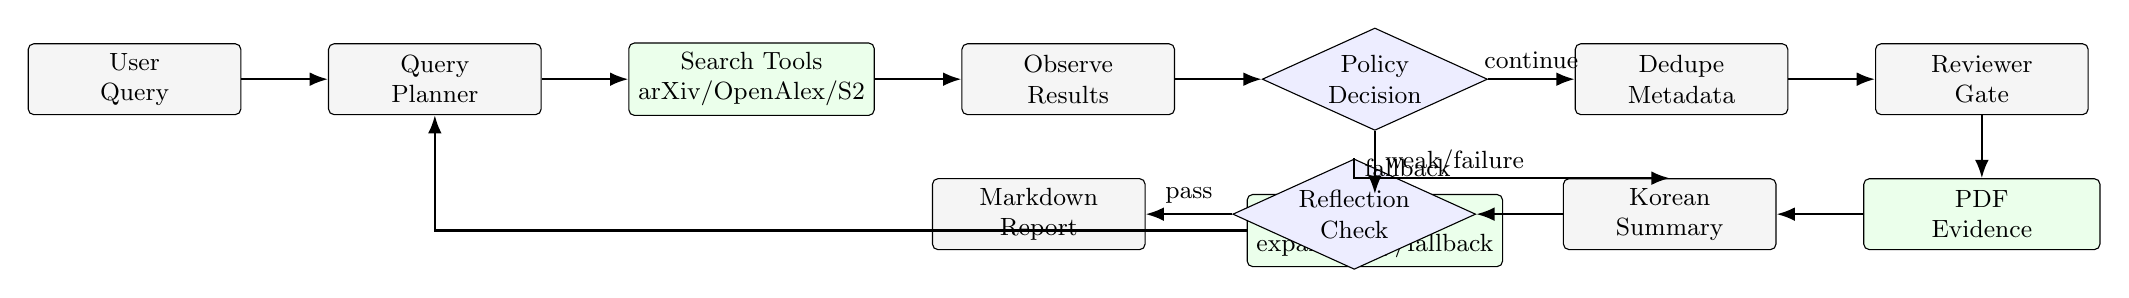
\begin{tikzpicture}[
      font=\small,
      box/.style={draw, rounded corners=2pt, align=center, minimum width=27mm, minimum height=9mm, fill=gray!8},
      decision/.style={draw, diamond, aspect=2.2, align=center, inner sep=1.5pt, fill=blue!7},
      action/.style={draw, rounded corners=2pt, align=center, minimum width=30mm, minimum height=9mm, fill=green!8},
      arrow/.style={-Latex, thick},
      node distance=8mm and 11mm
    ]
      \node[box] (query) {User\\Query};
      \node[box, right=of query] (planner) {Query\\Planner};
      \node[action, right=of planner] (search) {Search Tools\\arXiv/OpenAlex/S2};
      \node[box, right=of search] (observe) {Observe\\Results};
      \node[decision, right=of observe] (policy) {Policy\\Decision};
      \node[action, below=of policy] (recover) {Recovery\\expand/skip/fallback};
      \node[box, right=of policy] (dedupe) {Dedupe\\Metadata};
      \node[box, right=of dedupe] (review) {Reviewer\\Gate};
      \node[action, below=of review] (pdf) {PDF\\Evidence};
      \node[box, left=of pdf] (summary) {Korean\\Summary};
      \node[decision, left=of summary] (reflect) {Reflection\\Check};
      \node[box, left=of reflect] (report) {Markdown\\Report};

      \draw[arrow] (query) -- (planner);
      \draw[arrow] (planner) -- (search);
      \draw[arrow] (search) -- (observe);
      \draw[arrow] (observe) -- (policy);
      \draw[arrow] (policy) -- node[above]{continue} (dedupe);
      \draw[arrow] (policy) -- node[right]{weak/failure} (recover);
      \draw[arrow] (recover.west) -| (planner.south);
      \draw[arrow] (dedupe) -- (review);
      \draw[arrow] (review) -- (pdf);
      \draw[arrow] (pdf) -- (summary);
      \draw[arrow] (summary) -- (reflect);
      \draw[arrow] (reflect) -- node[above]{pass} (report);
      \draw[arrow] (reflect.north) |- node[pos=0.24, right]{fallback} (summary.north);
    \end{tikzpicture}
  }
  \caption{PaperPilot의 agentic curation workflow. 검색 결과와 실패 상태를 관찰한 뒤 policy decision이 다음 행동을 결정하고, 복구 행동은 다시 planning/search 단계로 되돌아간다.}
  \label{fig:workflow}
\end{figure*}

\subsection{Workflow Overview}

전체 workflow는 Fig.~\ref{fig:workflow}와 같이 실행된다. 먼저 QueryPlannerAgent는 원본 query를 유지하면서 deterministic rule 기반 query variant를 생성한다. SearcherAgent는 arXiv, OpenAlex, Semantic Scholar 중 사용자가 선택한 source를 호출하고 source별 결과 수, 오류, rate limit, 후보 부족 여부를 기록한다. 이후 CurationPolicyAgent는 \texttt{continue}, \texttt{expand\_query}, \texttt{try\_broad\_search}, \texttt{skip\_rate\_limited\_source}, \texttt{use\_abstract\_fallback}, \texttt{use\_heuristic\_summary\_fallback}, \texttt{stop\_with\_failure\_analysis} 중 하나를 선택한다.

검색 후보는 DOI, arXiv ID, normalized title 기준으로 중복 제거된다. ReviewerAgent는 relevance, novelty, experimental strength를 점수화하고 threshold를 통과한 후보만 선택한다. 선택 논문은 PDF extractor를 통해 제한된 page/character budget 안의 evidence를 추출한다. 마지막으로 SummarizerAgent는 한국어 5단 요약을 생성하고 reflection rule로 품질을 확인한 뒤 MarkdownPublisher가 Search Attempts, Agent Trace, Selected Papers, Failure Analysis를 포함한 report를 저장한다.

\subsection{Agents}

QueryPlannerAgent는 사용자가 입력한 query를 4--6개 이하의 bounded variant로 확장한다. 예를 들어 \texttt{diffusion language model unlearning}은 \texttt{DLM unlearning}, \texttt{discrete diffusion language model unlearning}, \texttt{language model unlearning} 등으로 확장된다. 이 과정은 LLM을 사용하지 않으므로 비용이 들지 않는다.

SearcherAgent는 source별 search tool을 호출하고 결과 수와 오류를 SearchAttempt로 기록한다. 또한 multi-source 결과를 중복 제거하여 reviewer가 볼 candidate pool을 만든다. CurationPolicyAgent는 관찰된 상태를 recovery action으로 변환한다. 기본 모드는 deterministic policy이며, 선택적으로 hybrid advisor를 붙일 수 있다. 프로젝트의 평가와 데모에서는 비용 통제를 위해 deterministic policy를 기본으로 사용한다.

ReviewerAgent는 후보 논문을 relevance, novelty, experimental strength로 점수화한다. 이는 전문가 판단을 대체하기 위한 것이 아니라, 약한 후보를 요약 단계로 넘기지 않기 위한 lightweight gate이다. SummarizerAgent는 heuristic, OpenAI, FactChat backend를 지원한다. LLM backend가 가능하면 structured summary를 생성하고, API key가 없거나 실패하면 heuristic fallback을 사용한다. OpenAI backend는 Structured Outputs~\cite{openai-structured-outputs}를 사용하고, FactChat backend는 Gateway API~\cite{factchat-gateway}를 OpenAI-compatible chat interface로 호출한다.

\subsection{Tools and External Actions}

PaperPilot은 arXiv API~\cite{arxivapi}, OpenAlex Works API~\cite{openalex}, Semantic Scholar Academic Graph API~\cite{semanticscholar}, PDF extractor, FactChat/OpenAI summary backend를 도구로 사용한다. Google Scholar는 자동 scraping 대상에서 제외하였다. 대신 \texttt{--scholar-links} 옵션으로 수동 확인 링크만 제공한다. 이는 안정성과 재현성을 우선한 설계 선택이다.

\section{Implementation}

PaperPilot은 Python package와 CLI entrypoint로 구현되었다. 주요 명령은 \texttt{curate}, \texttt{eval}, \texttt{models}, \texttt{credits}이다. \texttt{curate}는 실제 논문 큐레이션 workflow를 실행하고, \texttt{eval}은 baseline과 agentic 조건을 반복 가능한 시나리오에서 비교한다. \texttt{models}와 \texttt{credits}는 FactChat Gateway 사용 시 사용 가능한 모델과 credit 상태를 확인하기 위한 보조 명령이다.

비용 통제를 위해 \texttt{--cost-profile} 옵션을 제공한다. \texttt{dev} profile은 \texttt{top-k 1}, PDF 8 pages / 24000 chars, \texttt{gpt-5.4-nano}, \texttt{summary-detail deep}을 기본으로 사용한다. \texttt{balanced}와 \texttt{final} profile은 더 많은 PDF budget과 summary detail을 사용한다. 개발과 fixture 평가에서는 heuristic summary를 사용하여 API 비용 없이 workflow를 검증할 수 있다.

Agentic behavior는 \texttt{--agentic-mode}로 제어한다. \texttt{off}는 baseline에 가까운 단일 pass 실행이고, \texttt{policy}는 deterministic observe-decide-act loop를 사용한다. \texttt{hybrid}는 LLM advisor를 사용할 수 있지만, policy guardrail이 허용한 action만 적용한다.

Report artifact는 발표와 분석을 위해 의도적으로 자세하게 기록한다. 각 report는 \texttt{Presentation Highlights}, \texttt{Project Alignment}, \texttt{Search Attempts}, phase별 \texttt{Agent Trace}, \texttt{Selected Papers}, zero-selected 시 \texttt{Failure Analysis}를 포함한다. 이 구조는 최종 발표에서 시스템이 어떻게 판단하고 행동했는지 설명하기 위한 evidence 역할을 한다.

\section{Results and Evaluation}

평가는 비용 없는 fixture mode를 중심으로 수행하였다. fixture mode는 실제 검색 recall을 측정하기보다는 시스템 행동이 반복 가능하게 작동하는지 검증하기 위한 모드이다. 평가 조건은 baseline과 agentic으로 나누었다. Baseline은 arXiv only, query expansion off, PDF off, heuristic summary, agentic mode off 설정이다. Agentic 조건은 arXiv/OpenAlex 기반 multi-source search, query expansion basic, PDF evidence on, reflection/fallback on, agentic mode policy 설정이다.

평가 시나리오는 세 가지이다. \texttt{multimodal\_rag}는 멀티모달 RAG와 document retrieval query expansion을 검증한다. \texttt{dlm\_unlearning}은 좁은 diffusion language model 표현에서 broader language model unlearning 표현으로 회복하는지 본다. \texttt{agentic\_ai\_evaluation}은 benchmark/evaluation 성격의 논문을 선호하는지 확인한다.

\subsection{Fixture Evaluation}

Table~\ref{tab:fixture-results}는 \texttt{paperpilot eval --mode fixture --all} 실행 결과이다.

\begin{table*}[t]
  \centering
  \caption{Fixture evaluation results. Baseline은 단일 arXiv 검색에 가깝고, agentic 조건은 query expansion, multi-source search, PDF evidence, reflection을 사용한다.}
  \label{tab:fixture-results}
  \small
  \begin{tabular}{llrrrrrrr}
    \toprule
    Scenario & Condition & Selected & Attempts & Replans & Deduped & PDF & Rel. & Reflect \\
    \midrule
    multimodal\_rag & baseline & 1 & 1 & 0 & 0 & 0.00 & 1.000 & 1.00 \\
    multimodal\_rag & agentic & 2 & 12 & 5 & 3 & 0.50 & 1.000 & 1.00 \\
    dlm\_unlearning & baseline & 0 & 1 & 0 & 0 & 0.00 & 0.000 & 0.00 \\
    dlm\_unlearning & agentic & 2 & 12 & 5 & 7 & 0.50 & 1.000 & 1.00 \\
    agentic\_ai\_evaluation & baseline & 1 & 1 & 0 & 0 & 0.00 & 1.000 & 1.00 \\
    agentic\_ai\_evaluation & agentic & 2 & 8 & 3 & 1 & 0.50 & 1.000 & 1.00 \\
    \bottomrule
  \end{tabular}
\end{table*}

가장 중요한 결과는 \texttt{dlm\_unlearning} 시나리오이다. baseline은 원본 query와 arXiv-only 설정에서 선택 논문을 찾지 못했지만, agentic 조건은 query expansion과 multi-source search를 통해 2개 후보를 선택하였다. 이는 PaperPilot의 핵심 가설인 ``검색 실패를 관찰하고 query/source 전략을 바꾸면 후보 회복이 가능하다''를 fixture 환경에서 보여준다.

다른 두 시나리오에서도 agentic 조건은 더 많은 search attempt와 replan을 수행했고, 중복 제거와 PDF evidence extraction을 기록했다. 이는 agentic 조건이 단순히 더 많은 기능을 켠 것이 아니라, 검색과 evidence 수집 과정을 관찰 가능한 trace로 남긴다는 점에서 baseline과 다르다.

\subsection{Live-Style Case Study}

라이브형 데모는 \texttt{diffusion language model unlearning} query로 수행하였다. 실행 설정은 arXiv와 OpenAlex를 source로 사용하고, PDF evidence를 활성화하며, \texttt{cost-profile dev}, \texttt{agentic-mode policy}, heuristic summary를 사용하였다.

생성된 report는 8 search attempts, 4 query variants, 2 sources, 11 duplicate merges, 20 unique candidates, 1 selected paper, 1/1 PDF evidence extraction success, 1/1 summary reflection pass를 기록했다. 초기 query인 \texttt{diffusion language model unlearning}은 arXiv에서 0개 결과를 반환했다. 그러나 OpenAlex는 9개 후보를 반환했고, 이후 \texttt{DLM unlearning}, \texttt{discrete diffusion language model unlearning}, \texttt{language model unlearning} query variant가 추가로 시도되었다. trace에는 \texttt{expand\_query} decision이 4회 기록되었다. 최종적으로 ReviewerAgent는 20개 unique candidate 중 4개가 relevance threshold 0.8을 통과했다고 판단했고, top-k 설정에 따라 1개 논문을 선택했다.

이 case study는 발표 데모에 적합하다. 완벽한 성공만 보여주는 것이 아니라, 좁은 query에서 일부 source가 실패하고, agent가 query를 확장하며, 중복 제거와 reviewer gate를 거쳐 근거 기반 report를 생성하는 과정을 보여주기 때문이다.

\subsection{Additional Live Evaluation}

최종 제출 전 live behavior를 더 확인하기 위해 세 개 시나리오를 실제 arXiv/OpenAlex 호출로 다시 평가하였다. 이 평가는 API 비용을 줄이기 위해 heuristic summary를 사용했으며, agentic 조건은 \texttt{cost-profile dev}와 \texttt{agentic-mode policy}를 사용하였다. 결과는 Table~\ref{tab:live-results}와 같다.

\begin{table*}[t]
  \centering
  \caption{Additional live evaluation with arXiv/OpenAlex. Fixture 결과와 달리 live 결과는 외부 API 상태와 최신 색인에 영향을 받는다.}
  \label{tab:live-results}
  \small
  \begin{tabular}{llrrrrrr}
    \toprule
    Scenario & Condition & Selected & Attempts & Replans & PDF & Rel. & Reflect \\
    \midrule
    multimodal\_rag & baseline & 1 & 1 & 0 & 0.00 & 1.000 & 1.00 \\
    multimodal\_rag & agentic & 1 & 2 & 0 & 0.00 & 1.000 & 1.00 \\
    agentic\_ai\_evaluation & baseline & 1 & 1 & 0 & 0.00 & 1.000 & 1.00 \\
    agentic\_ai\_evaluation & agentic & 1 & 2 & 0 & 1.00 & 1.000 & 1.00 \\
    dlm\_unlearning & baseline & 0 & 1 & 0 & 0.00 & 0.000 & 0.00 \\
    dlm\_unlearning & agentic & 1 & 2 & 0 & 0.00 & 1.000 & 1.00 \\
    \bottomrule
  \end{tabular}
\end{table*}

Live 결과에서는 \texttt{multimodal\_rag}와 \texttt{agentic\_ai\_evaluation}의 baseline도 이미 1개 후보를 선택했기 때문에 selected count 자체의 향상은 작았다. 그러나 \texttt{agentic\_ai\_evaluation}에서는 agentic 조건이 PDF evidence success 1.00을 기록해 summary grounding을 추가했다. \texttt{dlm\_unlearning}에서는 baseline이 0개를 선택한 반면 agentic 조건은 1개를 선택해, 좁은 query 실패에서 multi-source agentic setting이 후보를 회복하는 case를 다시 확인했다.

\section{Discussion}

PaperPilot의 장점은 LLM 출력 자체보다 workflow의 관찰 가능성에 있다. 대부분의 paper summarization demo는 최종 요약만 보여주지만, PaperPilot은 왜 어떤 검색어를 시도했는지, 어떤 source가 실패했는지, 왜 후보가 선택되었는지, PDF evidence가 있었는지, summary reflection이 통과했는지를 report에 남긴다. 따라서 사용자는 결과를 그대로 믿기보다, system decision을 검토하고 다음 검색 전략을 조정할 수 있다.

또한 비용을 통제한 설계가 중요하다. Query expansion과 policy decision은 deterministic rule로 처리되며, LLM은 summary wording quality를 높이는 선택적 backend로만 사용된다. 이는 과제의 ``실제 문제를 위해 작동하는 Agentic System'' 목표에 맞게, 모델 데모보다 반복 가능한 workflow를 우선한 설계이다.

다만 fixture evaluation은 실제 검색 품질을 측정하지 않는다. fixture는 시스템 행동의 재현성을 검증하는 용도이며, 실제 recall과 precision은 live search의 API coverage, rate limit, publication timing에 영향을 받는다. 따라서 최종 발표에서는 fixture table과 함께 live-style case study를 같이 제시해야 한다.

\section{Limitations}

첫째, ReviewerAgent의 점수화는 lightweight deterministic scoring이다. relevance, novelty, experimental strength를 빠르게 비교할 수 있지만, 전문가가 논문의 기여를 최종 판단하는 과정을 대체하지 않는다.

둘째, 외부 search API의 coverage와 rate limit에 영향을 받는다. Semantic Scholar는 API key가 없으면 429 rate limit이 발생할 수 있고, OpenAlex와 arXiv도 검색 방식에 따라 결과가 달라질 수 있다. PaperPilot은 이러한 실패를 trace에 남기고 recovery를 수행하지만, 모든 관련 논문을 보장하지는 않는다.

셋째, PDF extraction은 표, 수식, 다단 레이아웃, 스캔 문서에서 정보를 놓칠 수 있다. 현재 시스템은 page와 character budget 안에서 추출한 text evidence에 의존하므로, 정량 결과와 limitation은 본문 후반부나 appendix까지 확인해야 할 수 있다.

넷째, heuristic summary는 비용 없이 실행 가능하지만 문장 품질과 domain-specific nuance가 LLM summary보다 약하다. FactChat 또는 OpenAI backend를 사용하면 한국어 요약 품질은 개선될 수 있으나, credit cost와 evidence validation 문제가 함께 생긴다.

\section{Conclusion}

PaperPilot은 최신 논문 탐색이라는 반복적 연구 작업을 agentic workflow로 구성한 시스템이다. 단순히 논문을 요약하는 것이 아니라, 검색 결과를 관찰하고, query를 확장하고, source 실패를 회복하고, 중복을 제거하고, reviewer gate와 PDF evidence를 거쳐 report를 생성한다. fixture 평가와 live-style case study는 baseline보다 agentic 조건이 실패 회복과 evidence tracking을 더 잘 보여줌을 확인했다. 향후에는 reviewer scoring을 더 정교화하고, live evaluation dataset을 확장하며, 최종 보고서용 LLM summary validation을 강화할 계획이다.

\bibliographystyle{ACM-Reference-Format}
\bibliography{references}

\end{document}
